% Provenance (never printed): old seconde/premiere S material on soil as a
% slowly renewed resource (alteration of rocks, clays, the clay--humus
% complex, soil erosion); see sources/book2/PROVENANCE.md. Rates are the
% medians of Montgomery (2007), computed in figdata/grade-10/soil_rates.py.
\chapter{土壤：形成缓慢的资源}\label{ch:g10:soil-formation}

湿润热带地区的山坡被公路切开，切面上露出一面红色土壁，
高度是人身高的数倍。坡脚处的岩石仍可辨认，
颜色发白、带有条纹，质地却十分松软，
用手指一捏即碎，仍可见原岩的颗粒与条带。
向上依次变为斑驳的黏土、一层坚硬的红色层，再变为
根系所在的薄层土壤。整面墙原本是完整的基岩：
它就是岩石本身，只是被水和空气原地缓慢改造。土壤是
陆地上所有植物及几乎所有人的食物都依托其生长，它正是这种岩柱的顶部。
本章阐明岩石如何变为土壤、哪些化学过程起作用、
气候如何决定其快慢，以及为何形成缓慢的土壤会
迅速流失。

\begin{omfigure}
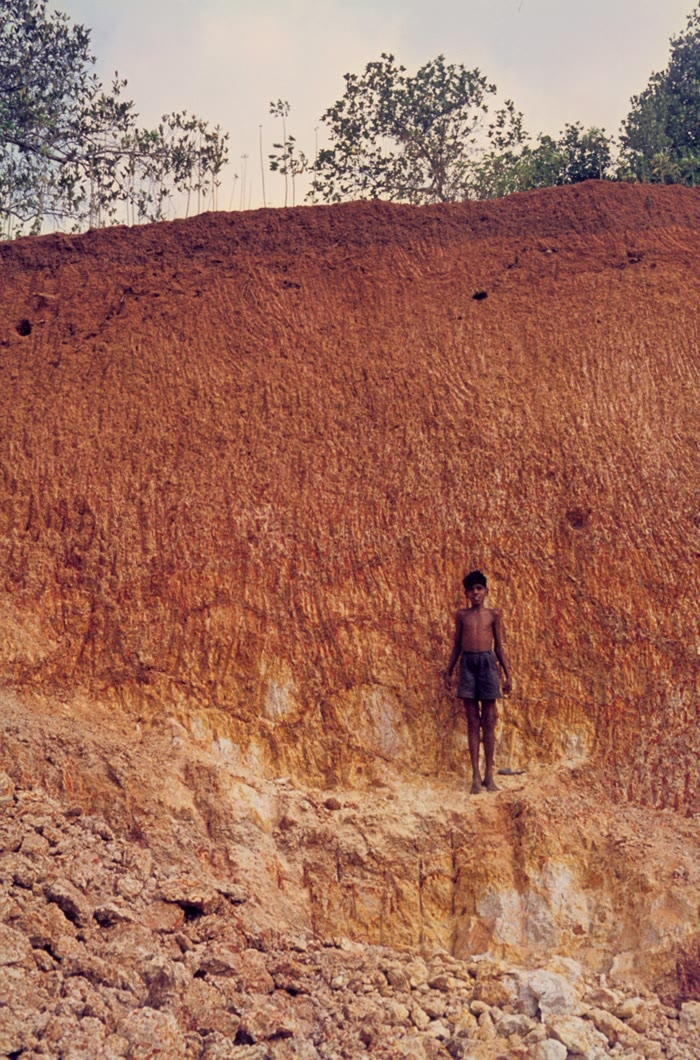
\includegraphics[height=8.5cm]{images/book2/g10-laterite-kerala.jpg}

{\small 印度南部喀拉拉邦花岗质片麻岩上的风化剖面：底部为斑驳的、已分解的岩石；
其上为棕色、弱硬化的\omterm{def:g10:soil-formation:laterite}{红土}，其上覆一层薄土壤。
图中男孩给出比例尺。照片：Werner
Schellmann, 1969（CC~BY-SA~2.5）。}
\end{omfigure}

\begin{recall}
风化使岩石原地破碎；侵蚀将碎屑搬运走，
沉积则将其堆积于别处（第 1 册，五年级）。岩石由矿物组成，
如花岗岩中的石英、长石和云母（第 1 册，
六年级）。土壤是由矿物颗粒、腐殖质、水、空气和生物体组成的活性层；
分解者将死亡物质转化为腐殖质；土壤通常按其
层次，即土层（生物学教材）。氧化过程中，物质
失去电子，常与氧结合（化学教材）。
\end{recall}

\section{从岩石到土壤}

物理风化——冰劈、冷热交替、植物根系——
在不改变矿物组成的情况下将岩石破碎成块。\omterm{def:g10:soil-formation:chemical-weathering}{化学风化}
则改变矿物本身。二者长期共同作用，使坚硬基岩的顶部
转变为松散的覆盖层，随风化向下推进而增厚，
不断侵入下方的岩石。

\begin{definition}[母岩；腐岩]\label{def:g10:soil-formation:weathering-profile}
土壤的\emph{母岩}\index{母岩}是指形成其
矿物部分的岩石。\emph{腐岩}\index{腐岩}是指
原地经风化分解、质地松软如土，仍保留着
母岩的颗粒与结构。\emph{风化剖面}指
由新鲜岩石经腐岩直至顶部土壤的整段柱状序列。
\end{definition}
% ledger: usgs:saprolite

\omterm{def:g10:soil-formation:weathering-profile}{腐岩}可以很厚。在美国东部阿巴拉契亚山脉东侧的起伏丘陵之下，
厚度在某些地方可达约
\qty{46}{m}（150 英尺），但厚度因地而异，变化很大；
土壤只是其上部。
% ledger: usgs:saprolite

\begin{omfigure}
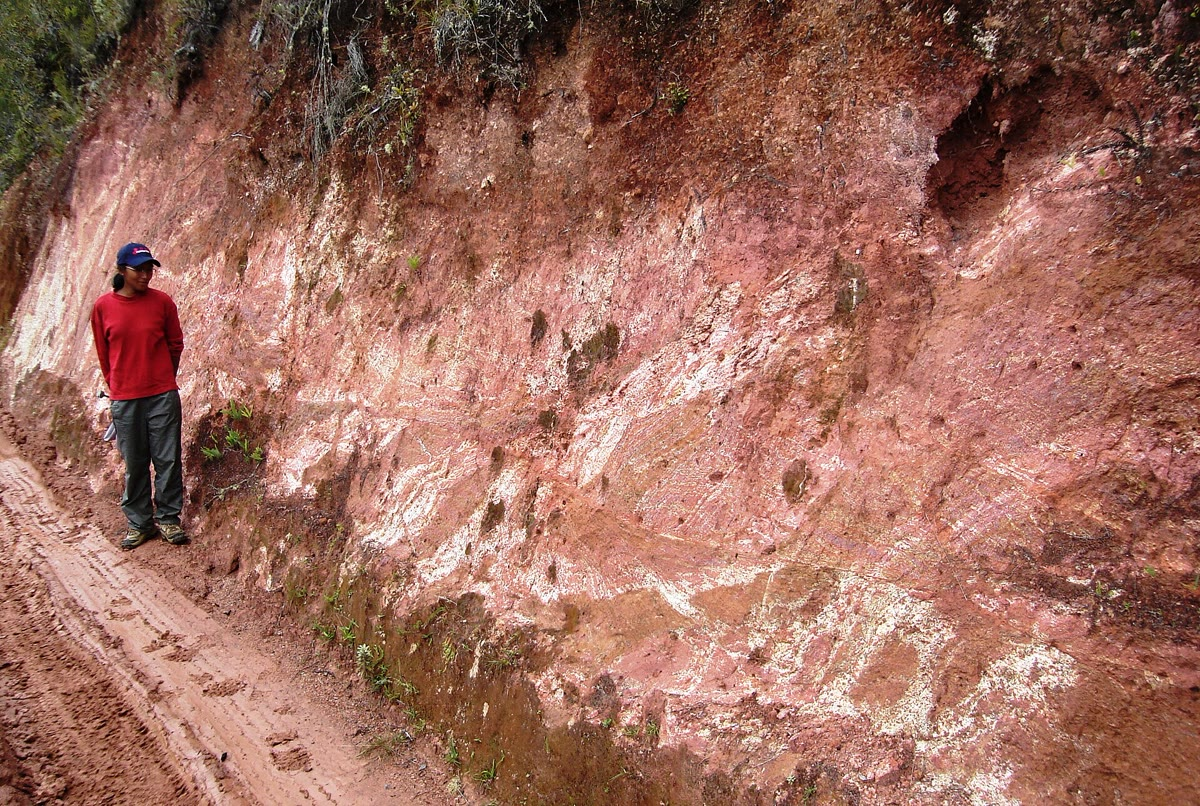
\includegraphics[width=0.8\linewidth]{images/book2/g10-saprolite-madagascar.jpg}

{\small 马达加斯加中部公路切面中的\omterm{def:g10:soil-formation:weathering-profile}{腐岩}：古老的片麻岩，
原地分解，其条带以白色黏土条纹的形式
嵌于红色土壤中。照片：Diorit（CC~BY-SA~3.0）。}
\end{omfigure}

\begin{omfigure}
\begin{tikzpicture}[font=\footnotesize]
  % humid tropical column
  \begin{scope}
    \fill[omThm!45!brown!60] (0,5.4) rectangle (1.8,6.0);
    \fill[omThm!70!orange!70] (0,4.2) rectangle (1.8,5.4);
    \fill[omThm!25!orange!35] (0,1.2) rectangle (1.8,4.2);
    \foreach \y in {1.5,2.1,2.7,3.3,3.9} \draw[white!80!black, thick] (0.1,\y) -- (1.7,\y+0.15);
    \fill[black!30] (0,0) rectangle (1.8,1.2);
    \foreach \x/\y in {0.3/0.3,0.9/0.7,1.4/0.2,0.5/0.9,1.2/1.0} \draw[black!55] (\x,\y) -- ++(0.2,0.08);
    \draw[black!60] (0,0) rectangle (1.8,6.0);
    \node[anchor=north, align=center] at (0.9,-0.1) {湿润热带};
  \end{scope}
  % temperate column
  \begin{scope}[xshift=3.2cm]
    \fill[omThm!45!brown!60] (0,2.2) rectangle (1.8,2.6);
    \fill[omThm!25!orange!35] (0,1.2) rectangle (1.8,2.2);
    \foreach \y in {1.5,1.9} \draw[white!80!black, thick] (0.1,\y) -- (1.7,\y+0.15);
    \fill[black!30] (0,0) rectangle (1.8,1.2);
    \foreach \x/\y in {0.3/0.3,0.9/0.7,1.4/0.2,0.5/0.9,1.2/1.0} \draw[black!55] (\x,\y) -- ++(0.2,0.08);
    \draw[black!60] (0,0) rectangle (1.8,2.6);
    \node[anchor=north, align=center] at (0.9,-0.1) {温带 \\气候};
  \end{scope}
  % labels
  \draw[black!50] (5.3,5.7) -- (2.0,5.7); \node[anchor=west] at (5.4,5.7) {土壤};
  \draw[black!50] (5.3,4.8) -- (2.0,4.8); \node[anchor=west, align=left] at (5.4,4.8) {红土：红色，富含铁 \\和铝的氧化物};
  \draw[black!50] (5.3,3.4) -- (2.0,3.4); \node[anchor=west, align=left] at (5.4,3.4) {腐岩：岩石原地分解 \\结构保留};
  \draw[black!50] (5.3,0.6) -- (5.0,0.6); \node[anchor=west] at (5.4,0.6) {新鲜母岩};
\end{tikzpicture}

{\small 同一岩石上的两种风化剖面（示意图，不按比例）：
在炎热潮湿的气候下，剖面厚得多，顶部为
\omterm{def:g10:soil-formation:laterite}{红土}；温带气候下，较薄的\omterm{def:g10:soil-formation:weathering-profile}{腐岩}承载着土壤。}
\end{omfigure}

\section{化学风化}

\begin{definition}[化学风化]\label{def:g10:soil-formation:chemical-weathering}
\emph{化学风化}\index{化学风化}是指岩石矿物
与水及其所携带的气体发生反应而发生的转变，
所携带的气体为二氧化碳和氧气：部分矿物溶解，
另一些转变为在地表稳定存在的新矿物。
\end{definition}

雨水从空气中溶解少量二氧化碳，渗过土壤时溶解的量要多得多，
土壤中的根系与分解者在此呼出二氧化碳。其中一部分溶解的
气体生成碳酸，碳酸释放出氢离子：
\begin{center}
\ce{CO2 + H2O -> H+ + HCO3-}
\end{center}
这些氢离子作用于矿物。

\begin{definition}[水解]\label{def:g10:soil-formation:hydrolysis}
\emph{水解}\index{水解}是指硅酸盐矿物
受水及其氢离子作用而发生的\omterm{def:g10:soil-formation:chemical-weathering}{化学风化}：氢离子取代矿物中的金属离子，
这些金属离子进入溶液，矿物的其余部分则重组为
一种\omterm{def:g10:soil-formation:clay}{黏土矿物}。
\end{definition}

\begin{proposition}[长石的水解]\label{prop:g10:soil-formation:hydrolysis}
钾长石（正长石）\ce{KAlSi3O8}，经\omterm{def:g10:soil-formation:hydrolysis}{水解}转变为
\omterm{def:g10:soil-formation:clay}{黏土矿物}高岭石 \ce{Al2Si2O5(OH)4}；钾离子和溶解的
硅酸 \ce{H4SiO4} 被水带走：
\begin{center}
\ce{2 KAlSi3O8 + 2 H+ + 9 H2O -> Al2Si2O5(OH)4 + 2 K+ + 4 H4SiO4}
\end{center}
\end{proposition}
% ledger: webmineral:formulas

\begin{proof}[验算]
分别统计两边各元素的原子数。钾：2 与 2；铝：2 与 2。
硅：6 与 $2 + 4 = 6$。氧：$16 + 9 = 25$ 与 $9 + 16 = 25$。
氢：$2 + 18 = 20$ 与 $4 + 16 = 20$。电荷：$+2$ 与 $+2$。
\end{proof}

\begin{proposition}[方解石的溶解]\label{prop:g10:soil-formation:calcite}
方解石 \ce{CaCO3}，即石灰岩的矿物，在携带二氧化碳的水中
完全溶解，不留任何固体：
\begin{center}
\ce{CaCO3 + CO2 + H2O -> Ca^2+ + 2 HCO3-}
\end{center}
\end{proposition}
% ledger: webmineral:formulas

铁受风化的方式是第三种。岩石中的暗色矿物，例如
花岗岩中的黑云母，其中的铁以还原态 \ce{Fe^2+} 存在。水所携带的氧
气将其氧化，三价铁以不溶性氧化物的形式
残留下来：黄褐色的针铁矿 \ce{FeO(OH)} 和红色的赤铁矿
\ce{Fe2O3}。针铁矿的反应式为：
\begin{center}
\ce{4 Fe^2+ + O2 + 6 H2O -> 4 FeO(OH) + 8 H+}
\end{center}
这些氧化物使风化后的岩石和土壤呈黄色、褐色和红色。
% ledger: webmineral:formulas

并非所有矿物的风化速率都相同。在风化的花岗岩中，黑
云母生锈，长石变为黏土，而几乎不溶的石英颗粒
基本保持不变，最终成为沙。

\begin{example}[花岗岩的风化]\label{ex:g10:soil-formation:granite}
% ledger: webmineral:formulas (masses computed in figdata/grade-10/soil_rates.py)
一千克正长石含有 $1000/278.33 \approx \qty{3.59}{mol}$ 的
\ce{KAlSi3O8}。由方程式可知，两摩尔正长石生成一摩尔
高岭石：$3.59/2 \approx \qty{1.80}{mol}$，即 $1.80 \times 258.16
\approx \qty{464}{g}$ 的黏土。钾占正长石质量的 $14.05~\%$，
即 \qty{140.5}{g}，以及 $2 \times 3.59 = \qty{7.19}{mol}$ 的硅酸
进入溶液。由石英、长石和云母组成的花岗岩风化后，
留下沙（即石英）、黏土（由长石和云母而来）和铁的氧化物，
并将钾、钠、钙和硅酸输送到河流中。
\end{example}

\section{黏土与腐殖质}

\begin{definition}[黏土矿物]\label{def:g10:soil-formation:clay}
\emph{黏土矿物}\index{黏土矿物}是一种硅酸盐，由薄层状的
原子层相互叠置而成，经风化形成，呈薄片状，
远小于沙粒。高岭石就是其中之一。
\end{definition}
% ledger: webmineral:formulas

黏土薄片表面带负电荷，它们吸附
正离子——钾离子 \ce{K+}、钙离子 \ce{Ca^2+}、镁离子
\ce{Mg^2+}、铵离子 \ce{NH4+}——若不被吸附，这些离子便会
随雨水流失。腐殖质同样如此。黏土与腐殖质结合在一起，构成
\emph{黏土–腐殖质复合体}，即土壤中矿质营养的储存库：根系
释放氢离子，换取吸附在
片层上的钾或钙。

\begin{omfigure}
\begin{tikzpicture}[font=\footnotesize, >={Stealth[length=2mm]}]
  \foreach \y in {0,0.7,1.4} {
    \fill[omExo!35, draw=black!60] (0,\y) rectangle (7.2,\y+0.3);
    \foreach \x in {0.3,0.9,...,7.0} \node[font=\tiny, black!70] at (\x,\y+0.15) {$-$};
  }
  \foreach \x/\ion in {0.7/K^+, 1.9/Ca^{2+}, 3.1/K^+, 4.3/Mg^{2+}, 5.5/NH_4^+, 6.7/K^+} {
    \fill[omThm!20, draw=omThm!80!black] (\x,2.1) circle (0.4);
    \node[font=\scriptsize] at (\x,2.1) {$\mathrm{\ion}$};
  }
  \foreach \x in {1.3, 3.7, 6.1} \fill[omThm!20, draw=omThm!80!black] (\x,0.5) circle (0.17);
  \foreach \x in {2.5, 4.9} \fill[omThm!20, draw=omThm!80!black] (\x,1.2) circle (0.17);
  \node[anchor=north] at (3.6,-0.1) {黏土片层带负电，片层间夹有正离子};
  \node[anchor=south] at (3.1,2.5) {正离子吸附在表面};
  % root and exchange
  \draw[line width=2.2pt, brown!60!black] (9.6,3.4) .. controls (9.3,2.6) and (8.9,2.2) .. (8.1,2.0);
  \node[anchor=east] at (9.25,3.3) {根};
  \draw[->, omDef!80!black, thick] (8.0,2.2) .. controls (7.6,2.6) and (7.2,2.6) .. (6.95,2.3);
  \node[anchor=south, omDef!80!black] at (7.5,2.55) {释放 \ce{H+}};
  \draw[->, omThm!80!black, thick] (6.95,1.8) .. controls (7.3,1.5) and (7.7,1.6) .. (8.0,1.85);
  \node[anchor=north, omThm!80!black] at (7.8,1.55) {吸收 \ce{K+}};
\end{tikzpicture}

{\small 黏土–腐殖质复合体（示意图）：带负电的黏土片层
在表面及片层间吸附正离子；根系用
氢离子交换这些营养物质。}
\end{omfigure}

\section{土壤与气候}

\omterm{def:g10:soil-formation:chemical-weathering}{化学风化}需要水，与多数反应一样，温度升高时
进行得更快。在既炎热又潮湿的气候下，岩石分解得最深、最远：
长石完全转变为黏土，甚至大部分二氧化硅也被带走，
留下的物质富含最难溶的元素，
即铁和铝。

\begin{definition}[红土]\label{def:g10:soil-formation:laterite}
称\emph{红土}\index{红土}为一种深度风化的物质，形成于炎热潮湿的
气候，呈红色或棕色，主要由铁和铝的氧化物以及高岭石组成，
其中几乎所有可溶成分均已被移除。
\end{definition}

在全年大部分时间冰冻的寒冷气候下，以及
水分稀缺的干旱气候下，\omterm{def:g10:soil-formation:chemical-weathering}{化学风化}进行得很慢：土壤薄，
基岩就在近地表处。从两极到赤道，风化深度
在潮湿的热带森林下最大，而在
沙漠和极地地区最小。

\begin{omfigure}
\begin{tikzpicture}[font=\footnotesize]
  \fill[black!25] (0,-0.2) -- (0,-0.5) .. controls (1.5,-0.6) and (2.5,-1.4) .. (3.4,-1.2)
     .. controls (4.2,-1.0) and (4.6,-0.55) .. (5.2,-0.5) .. controls (6.0,-0.5) and (6.6,-1.6) .. (7.6,-3.0)
     .. controls (8.2,-3.6) and (9.0,-3.6) .. (10,-3.4) -- (10,-3.8) -- (0,-3.8) -- cycle;
  \fill[omThm!25!orange!35] (0,0) -- (10,0) -- (10,-3.4) .. controls (9.0,-3.6) and (8.2,-3.6) .. (7.6,-3.0)
     .. controls (6.6,-1.6) and (6.0,-0.5) .. (5.2,-0.5) .. controls (4.6,-0.55) and (4.2,-1.0) .. (3.4,-1.2)
     .. controls (2.5,-1.4) and (1.5,-0.6) .. (0,-0.5) -- cycle;
  \draw[black!60] (0,0) -- (10,0);
  \node[anchor=south] at (0.6,0.05) {极地};
  \node[anchor=south] at (3.2,0.05) {温带};
  \node[anchor=south] at (5.3,0.05) {沙漠};
  \node[anchor=south] at (6.8,0.05) {稀树草原};
  \node[anchor=south] at (9.0,0.05) {热带森林};
  \node[anchor=north] at (0.4,-3.85) {极};
  \node[anchor=north] at (9.6,-3.85) {赤道};
  \node[black!70] at (2.0,-2.6) {新鲜岩石};
  \node[black!80] at (8.35,-1.0) {风化岩石与土壤};
\end{tikzpicture}

{\small 从极地到赤道的风化深度（示意图，深度未按比例绘制）：
极地和沙漠气候下较薄，温带气候下中等，
潮湿的热带森林下最厚。}
\end{omfigure}

\section{形成缓慢，流失迅速}

土壤形成得有多快？土壤生成，即风化作用在剖面底部把岩石转变为土壤的速率，
已在世界许多地点测得；土壤从地表被侵蚀的速率亦然。
对这些测量结果加以汇总，
所得的典型（中位数）速率如下，
每一速率均以每年土壤的厚度表示。
% ledger: montgomery:rates

\begin{omfigure}
\begin{tikzpicture}
\begin{axis}[omrecord, width=0.82\linewidth, height=5.6cm, ymode=log, log origin=infty, ymin=0.005,
  ymax=5, ybar, bar width=16pt, xtick={0,1,2,3,4}, xmin=-0.6, xmax=4.6,
  xticklabels={{土壤 \\生成}, {原生植被下 \\侵蚀}, {地质 \\侵蚀}, {保护性 \\耕作}, {传统 \\翻耕}},
  xticklabel style={align=center, font=\scriptsize},
  ylabel={速率（\unit{mm} 每年）}, tick label style={font=\small}, label style={font=\small},
  nodes near coords, nodes near coords style={font=\scriptsize}, point meta=explicit symbolic]
\addplot[fill=omDef!45, draw=omDef!80!black] table[x=idx, y=rate_mm_yr, meta=rate_mm_yr] {figdata/out/grade-10-soil_rates-rates.dat};
\end{axis}
\end{tikzpicture}

{\small 全球测量汇总所得的土壤生成与侵蚀速率中位数，
以每年土壤的毫米数计（对数刻度：每一级为其下一级的十倍）。
数据来源：Montgomery（2007），
\emph{Proceedings of the National Academy of Sciences}。}
\end{omfigure}
% ledger: montgomery:rates

在原生植被下，土壤被侵蚀的速度与其形成速度大致相当，约为
\qty{0.02}{mm} 每年，即约六个世纪侵蚀一厘米。在传统翻耕下，
作物之间的地面裸露，侵蚀速率的中位数
为 \qty{1.5}{mm} 每年，是土壤生成速率的九十倍。在保护性耕作下，
土壤受扰动较少且保持覆盖，中位侵蚀速率
降至 \qty{0.08}{mm} 每年，更接近
土壤生成速率。
% ledger: montgomery:rates (ratios computed in figdata/grade-10/soil_rates.py)

\begin{method}[比较形成速率与侵蚀速率]\label{met:g10:soil-formation:rates}
\begin{enumerate}
  \item 将两种速率统一为同一单位（毫米每年）。
  \item 净流失量为侵蚀速率 $E$ 减去生成速率 $P$。
  \item 厚度为 $S$ 的土壤流失所需时间为 $T = S/(E - P)$ 年；若
        $E \le P$，则土壤未发生流失。
  \item 从零开始形成厚度为 $S$ 的土壤所需时间为 $S/P$ 年。
\end{enumerate}
\end{method}
% ledger: montgomery:lifetime

按这些速率，形成一米厚的土壤约需 $1000/0.017 \approx 59\,000$
年；而在传统翻耕下，这层土壤约
$1000/(1.537 - 0.017) \approx 660$ 年即可流失。就人类的时间尺度而言，土壤是一种
不可再生的资源。
% ledger: montgomery:rates, montgomery:lifetime

\begin{omfigure}
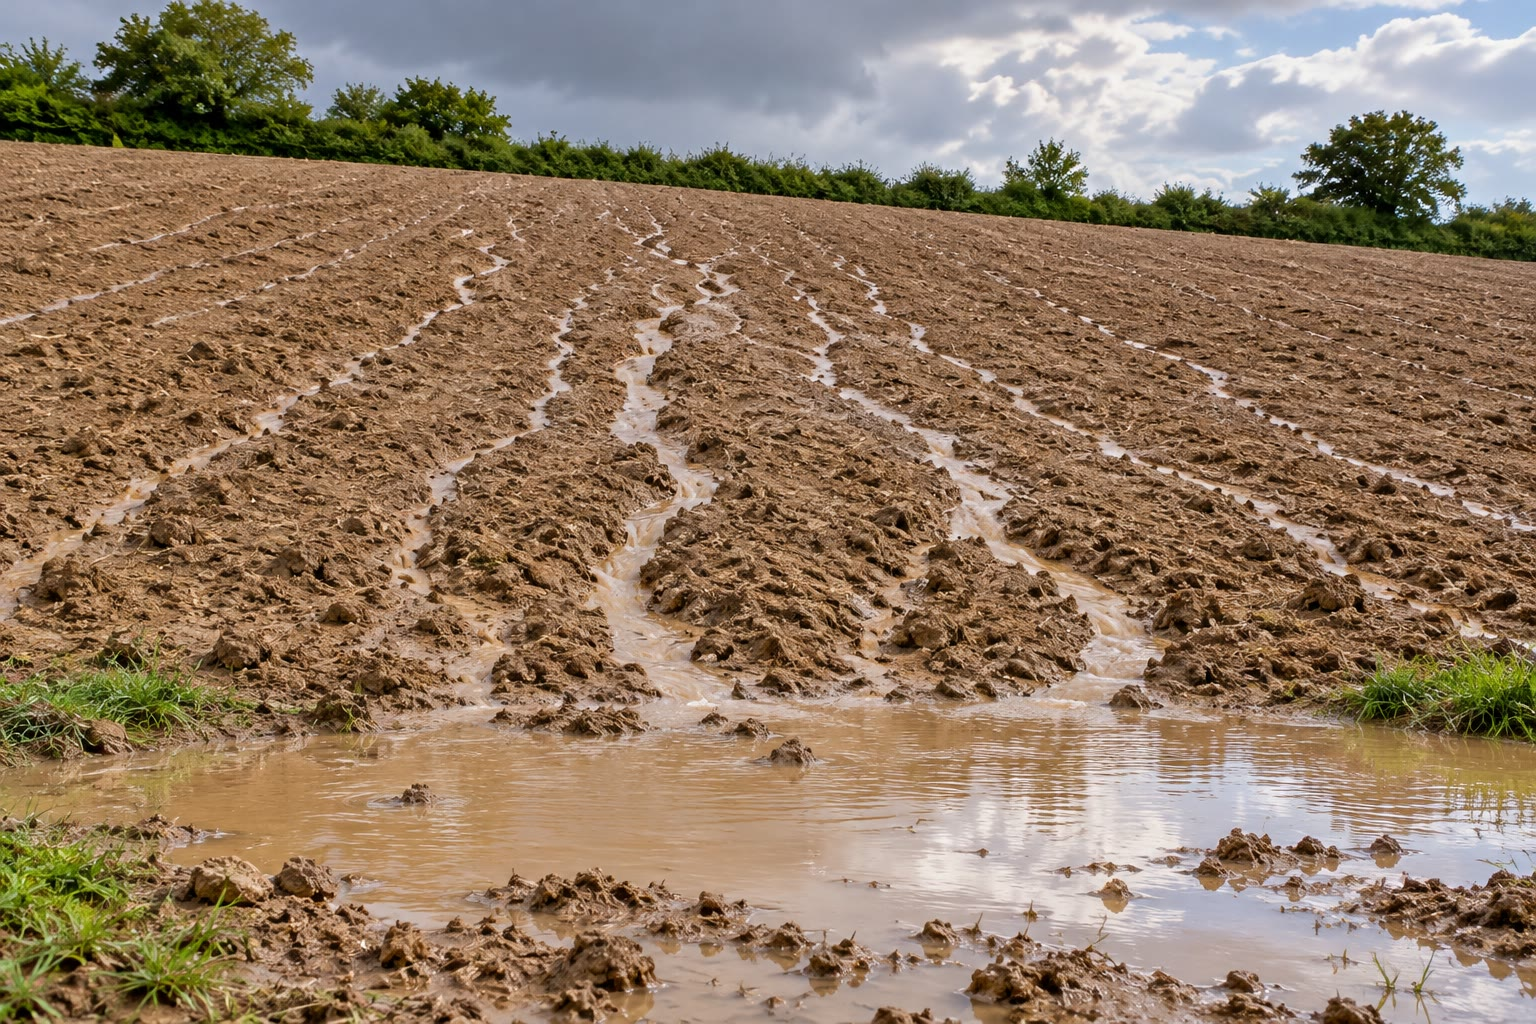
\includegraphics[width=0.72\linewidth]{images/book2/ai/g10-ploughed-rills.jpg}

{\small 暴雨过后的耕地：径流沿坡面冲出许多小
沟槽，即细沟，并将土壤冲入
坡脚处的泥水洼中。}
\end{omfigure}

\section{练习}

\begin{exercise}[$\star$]\label{exo:g10:soil-formation:1}
给出\omterm{def:g10:soil-formation:chemical-weathering}{化学风化}和\omterm{def:g10:soil-formation:hydrolysis}{水解}的定义。
\end{exercise}

\begin{exercise}[$\star$]\label{exo:g10:soil-formation:2}
什么是\omterm{def:g10:soil-formation:weathering-profile}{腐岩}？如何区分\omterm{def:g10:soil-formation:weathering-profile}{腐岩}与在
河流搬来的沙上形成的土壤？
\end{exercise}

\begin{exercise}[$\star$]\label{exo:g10:soil-formation:3}
写出花岗岩风化的产物：其三种
主要矿物各变成什么？
\end{exercise}

\begin{exercise}[$\star$]\label{exo:g10:soil-formation:4}
为什么风化岩和热带土壤常呈红色、黄色或棕色？
\end{exercise}

\begin{exercise}[$\star$]\label{exo:g10:soil-formation:5}
利用柱状图，给出常规耕作下土壤形成速率的中位数和
侵蚀速率的中位数，并算出
后者是前者的多少倍？
\end{exercise}

\begin{exercise}[$\star\star$]\label{exo:g10:soil-formation:6}
检验方解石溶解的方程式是否配平，逐一检查
每种元素及电荷是否守恒。
\end{exercise}

\begin{exercise}[$\star\star$]\label{exo:g10:soil-formation:7}
石灰岩完全溶解，花岗岩则留下沙和黏土，请解释
二者的差异，利用本章的两个反应加以说明。
\end{exercise}

\begin{exercise}[$\star\star$]\label{exo:g10:soil-formation:8}
解释黏土–腐殖质复合体如何在经雨水不断淋洗的
土壤中保留钾，以及根如何吸收它。
\end{exercise}

\begin{exercise}[$\star\star$]\label{exo:g10:soil-formation:9}
给出两个原因，说明\omterm{def:g10:soil-formation:laterite}{红土}为何在炎热潮湿的
气候下形成，而不在寒冷或干燥的气候下形成。
\end{exercise}

\begin{exercise}[$\star\star$]\label{exo:g10:soil-formation:10}
土壤形成速率的中位数为每年 \qty{0.017}{mm}。要形成
\qty{1}{cm}、\qty{30}{cm} 和 \qty{1}{m} 厚的土壤各需多长时间？
\end{exercise}

\begin{exercise}[$\star\star$]\label{exo:g10:soil-formation:11}
侵蚀速率常以每年每公顷土壤的质量表示。已知
土壤密度为 \qty{1200}{kg/m^3}，每年损失
\qty{1.5}{mm} 的土壤，在一公顷（\qty{10000}{m^2}）上相当于多少质量？
\end{exercise}

\begin{exercise}[$\star\star\star$]\label{exo:g10:soil-formation:12}
厚 \qty{46}{m} 的\omterm{def:g10:soil-formation:weathering-profile}{腐岩}形成于温带地区的丘陵之下。若风化作用以
每年 \qty{0.017}{mm} 的速率向岩石中推进，则形成该\omterm{def:g10:soil-formation:weathering-profile}{腐岩}需要多长时间？
这一结果对此类
地貌的年代有何启示？
\end{exercise}

\begin{exercise}[$\star\star\star$]\label{exo:g10:soil-formation:13}
写出书中给出的 \ce{Fe^2+} 氧化为针铁矿
的方程式并加以检验，然后写出并配平
\ce{Fe^2+} 借氧气和水氧化为赤铁矿 \ce{Fe2O3} 的方程式，同时释放 \ce{H+}。
\end{exercise}

\begin{exercise}[$\star\star\star$]\label{exo:g10:soil-formation:14}
保护性耕作下，侵蚀速率的中位数为
每年 \qty{0.082}{mm}。若土壤形成速率为每年 \qty{0.017}{mm}，则
损失 \qty{30}{cm} 的土壤需要多长时间？并与常规耕作进行比较。
\end{exercise}

\begin{exercise}[$\star\star\star$]\label{exo:g10:soil-formation:15}
某花岗岩中正长石的质量分数为 \qty{30}{\percent}。将
一吨该花岗岩中的正长石全部风化，可生成多少质量的
高岭石，又释放出多少质量的钾？
\end{exercise}

\section{问题：土壤的寿命}

\begin{problem}[{周末问题——从岩石到农田，再回到河流}]
\label{pb:g10:soil-formation:1}
% ledger: montgomery:rates, montgomery:lifetime, webmineral:formulas (values computed in figdata/grade-10/soil_rates.py)

\begin{center}
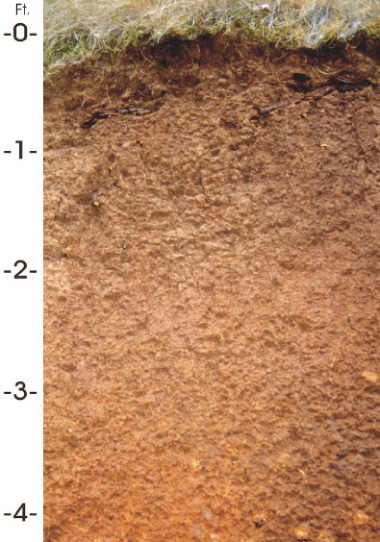
\includegraphics[height=6cm]{images/book2/g10-nrcs-jory-soil.jpg}

{\small 土壤剖面，左侧刻度以英尺为单位（\num{1}~英尺 =
\qty{0.3048}{m}）。照片：USDA Natural Resources Conservation Service
（公有领域）。}
\end{center}

\medskip
\noindent\textbf{第一部分——剖面。}
\begin{enumerate}
  \item 图片底部附近的刻度达到 4 英尺。该处
        深度是多少米？
  \item 顶部深色层约为半英尺。该层
        厚度为多少厘米？
  \item 是什么使这一顶层呈深色？
  \item 下方土壤呈红棕色。哪些矿物使其呈现这种
        颜色，这些矿物是如何形成的？
  \item 照片中能否看到\omterm{def:g10:soil-formation:weathering-profile}{母岩}？在图片底部
        以下，你预计会找到什么？
\end{enumerate}

\medskip
\noindent\textbf{第二部分——风化花岗岩的化学过程。}
\begin{enumerate}[resume]
  \item 写出正长石\omterm{def:g10:soil-formation:hydrolysis}{水解}的方程式。
  \item \qty{1}{kg} 正长石中含有多少摩尔
        （摩尔质量 \qty{278.33}{g/mol}）？
  \item 这些正长石能生成多少质量的高岭石（摩尔质量 \qty{258.16}{g/mol}）？
  \item 哪些物质随水流失？它们去向何处？
  \item 花岗岩中的石英发生了什么变化？
\end{enumerate}

\medskip
\noindent\textbf{第三部分——成土与侵蚀的较量。}
\begin{enumerate}[resume]
  \item 土壤以每年 \qty{0.017}{mm} 的速率形成。形成
        第一部分中的剖面需要多长时间？
  \item 常规耕作下，土壤以
        每年 \qty{1.537}{mm} 的速率被侵蚀，每年的净损失是多少？
  \item 第一部分中的剖面能维持多长时间？
  \item 比较第 11 题和第 13 题所求的两个时间。
  \item 在自然植被覆盖下，侵蚀速率为每年 \qty{0.013}{mm}。土壤
        是否仍在流失？
\end{enumerate}

\medskip
\noindent\textbf{第四部分——土壤的寿命。}
\begin{enumerate}[resume]
  \item 写出损失土壤所需的时间 $T$（土壤厚度为 $S$）
        关于 $S$、侵蚀速率 $E$ 和生成速率 $P$ 的函数表达式。
  \item 计算常规耕作下 $T$ 的值，取 $S = \qty{30}{cm}$。
  \item 计算保护性耕作下 $T$ 的值，取 $S = \qty{30}{cm}$，
        侵蚀速率为每年 \qty{0.082}{mm}。
  \item 为何可以说土壤是一种在人类
        时间尺度上不能再生的资源？
  \item 在常规耕作下，损失一米
        土壤需要多长时间？
\end{enumerate}
\end{problem}
